\paragraph{Question 1}

Vous trouverez sur le graphique ci-dessous une représentation du
polytope associé aux équations de $PL_0$ (aire située à la fois sous la courbe
bleue et sous la courbe rouge).

\begin{figure}[h!]
\centering
\begin{tikzpicture}[scale=1.2]
    \begin{axis}[title=PL, xlabel=x1, ylabel=x2]
      \addplot
        table[col sep=comma]{equ1.csv};
        \addplot
        table[col sep=comma]{equ2.csv};
        \addplot
        table[col sep=comma]{abs.csv};
        \addplot
        table[col sep=comma]{ord.csv};
        \legend{contrainte1, contrainte2}
    \end{axis}
\end{tikzpicture}
\caption{Polytope exercice 12}
\end{figure}

\paragraph{Question 2}
De manière graphique, on trouve environ $x_1 = 1.5$, $x_2 = 3$, $z = 6$.

\paragraph{Question 3}

Résolution du problème donné par la méthode du simplexe.

\begin{table}[h!]	
\centering
	\begin{tabular}{|c|c|c|c|c|c|}
	\hline
      & c & 2 & 1 & 0 & 0 \\ 
      \cline{2-6}
       &  & $x_{1}$ & $x_{2}$  & $x_{3}$  & $x_{4}$ \\
       \hline
   0 & $x_{3}$  $=$ 17 & 2 & 5 & 1 & 0 \\
      \hline
	0 & $x_{4}$ $=$ 10  & 3 & 2 & 0 & 1 \\
	  \hline
	 & Z($x$)$=$ 0 & -2 & -1 & 0 & 0\\
	  \hline
	\end{tabular}
\caption {Tableau 1 du simplex}	
\centering
	\begin{tabular}{|c|c|c|c|c|c|}
	\hline
      & c & 2 & 1 & 0 & 0 \\ 
      \cline{2-6}
       &  & $x_{1}$ & $x_{2}$  & $x_{3}$  & $x_{4}$ \\
       \hline
   0 & $x_{3}$  $=$ $\frac{31}{3}$ & 0 & $\frac{11}{3}$ & 1 & $\frac{-2}{3}$ \\
      \hline
	2 & $x_{1}$ $=$ $\frac{10}{3}$  & 1 & $\frac{2}{3}$ & 0 & $\frac{1}{3}$ \\
	  \hline
	 & Z($x$)$=$ $\frac{20}{3}$ & 0 & $\frac{1}{3}$ & 0 & $\frac{2}{3}$\\
	  \hline
	\end{tabular}
\caption {Tableau 2 du simplex}
\end{table}



\paragraph{Question 4, a) Branch and Bound}
\begin{itemize}
\item Nous utilisons la solution initiale suivante~:
\begin{equation}
\begin{cases}
x_1 = \frac{10}{3} \\
x_2 = 0 \\
x_3 = \frac{31}{3} \\
x_4 = 0 \\
z(x) = \frac{20}{3} \\
\end{cases}
\end{equation}
\item Nous procédons ensuite à la troncature suivante pour obtenir la
  borne inférieure de notre programme en nombres entiers.
\begin{equation}
\begin{cases}
x_1 = 3 \\
x_2 = 0 \\
z(x) = 2 \times 3 + 0 = 6 \\
\end{cases}
\end{equation}
\item Effectuons désormais un branchement sur $x_1$.
\end{itemize}
\vspace{0.5cm}
 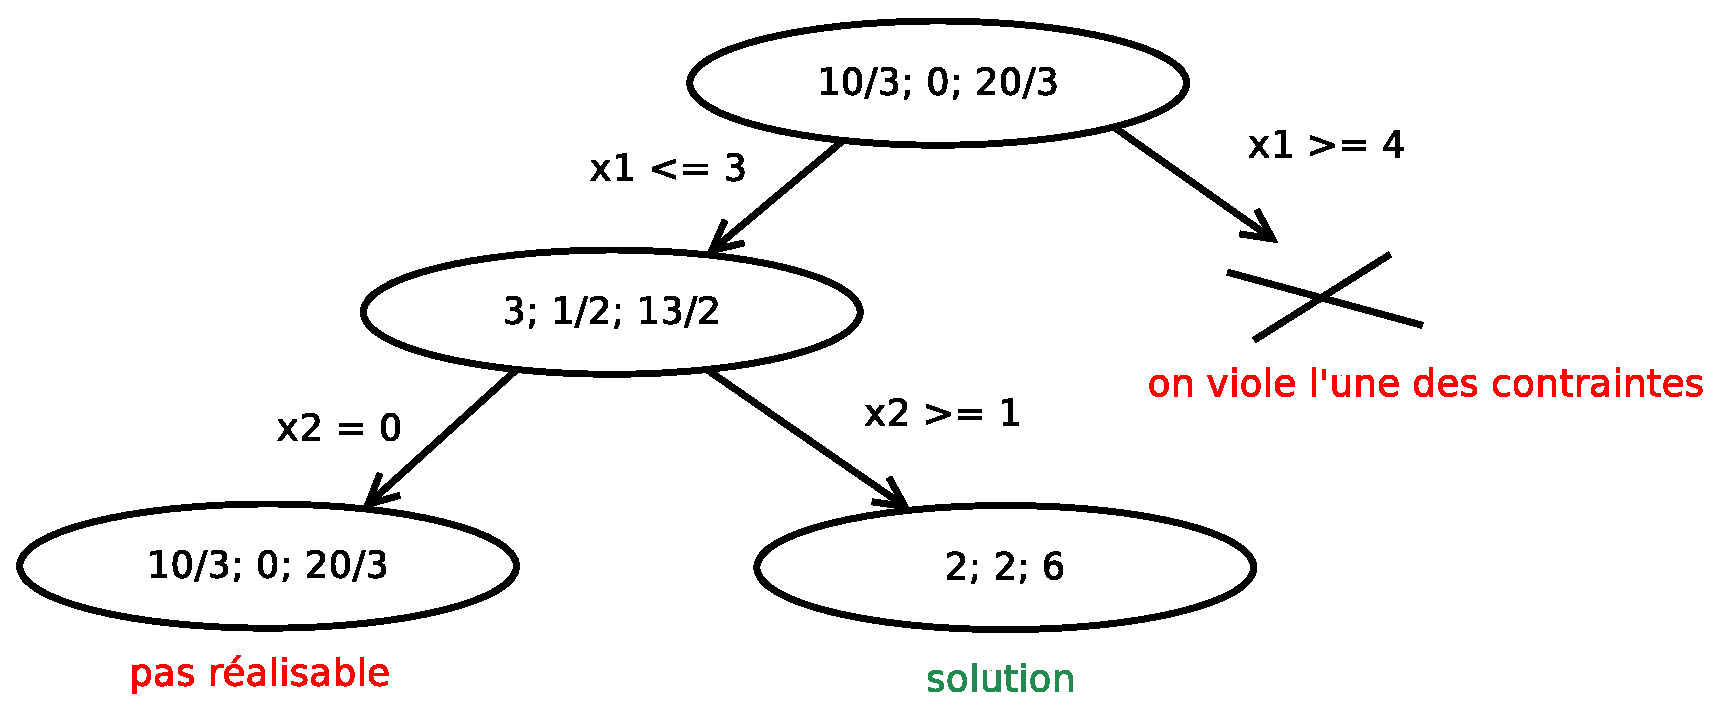
\includegraphics[height=60mm]{branchAndBound.eps}
\paragraph{Question 4, b) Branch and Cut}

Vous trouvez ci dessous les différents étapes des tableaux de la
méthode de Branch and Cut. \\
Les étapes intermédiaires sont les suivantes~:
\begin{itemize}
\item on commence par reprendre les résultats de la question
  concernant la résolution par le simplexe, puis l'on fixe la deuxième
  ligne, d'où $i = 2$.
\item $x_2$ et $x_4$ sont les variables qui ne sont pas en base. On
  peut donc écrire $\frac{2}{3} x_2 + \frac{1}{3} x_4 \geq
  \frac{1}{3}$.
\item Graphiquement, cela correspond à $x_1 \leq 3$ car on a 
\begin{equation}
\begin{cases}
2x_1 + 5x_2 + x_3  = 17 \\
3x_1 + 2x_2 + x_4  = 10 \\
\end{cases}
\\
\Rightarrow x_4  = 10 - 3x_1 - 2x_2 
\end{equation}
Ainsi, en remplaçant $x_4$ dans l'équation de l'item précédent, on a
\\
$\frac{2}{3}x_2 + \frac{1}{3}(10-3x_1-2x_2) \geq \frac{1}{3}$ \\
$\frac{2}{3}x_2 + \frac{10}{3} - x_1 - \frac{2}{3}x_2 \geq
\frac{1}{3}$ \\
$\frac{10}{3} - x_1 \geq \frac{1}{3}$ \\
$-x_1 \geq \frac{-9}{3} = -3$ \\
$\Rightarrow x_1 \leq 3$.
\item On rajoute la nouvelle contrainte obtenue dans notre tableau du
  simplexe, que nous résolvons alors par la méthode à deux phases.
\end{itemize}

TODO : étapes intermédiaires !!

\begin{table}[h!]	
\centering
	\begin{tabular}{|c|c|c|c|c|c|c|c|}
	\hline
      & c & 0 & 0 & 0 & 0 & 0 & -1 \\ 
      \cline{2-8}
       &  & $x_{1}$ & $x_{2}$  & $x_{3}$  & $x_{4}$ & $x_{5}$ & $y$ \\
       \hline
   0 & $x_{3}$  $=$ $\frac{31}{3}$ & 0 & $\frac{11}{3}$ & 1 & $\frac{-2}{3}$ & 0 & 0 \\
      \hline
	0 & $x_{1}$ $=$ $\frac{10}{3}$  & 1 & $\frac{2}{3}$ & 0 & $\frac{1}{3}$ & 0 & 0 \\
	  \hline
	  -1 & $y$ $=$ $\frac{1}{3}$  & 0 & $\frac{2}{3}$ & 0 & $\frac{1}{3}$ & -1 & 1 \\
	    \hline
	 $\frac{-1}{3}$ & Z($x$)$=$ 0 & 0 & $\frac{-2}{3}$ & 0 & $\frac{-1}{3}$ & 1 & 0\\
	  \hline
	\end{tabular}
\caption {Tableau 1 des coupes de Gomory}
\end{table}
\begin{table}[h!]	
\centering
	\begin{tabular}{|c|c|c|c|c|c|c|}
	\hline
      & c & 2 & 1 & 0 & 0 & 0 \\ 
      \cline{2-7}
       &  & $x_{1}$ & $x_{2}$  & $x_{3}$  & $x_{4}$ & $x_{5}$ \\
       \hline
   0 & $x_{3}$  $=$ $\frac{31}{3}$ & 0 & $\frac{11}{3}$ & 1 & $\frac{-2}{3}$ & 0 \\
      \hline
	2 & $x_{1}$ $=$ $\frac{10}{3}$  & 1 & $\frac{2}{3}$ & 0 & $\frac{1}{3}$ & 0 \\
	  \hline
	0 & $y$ $=$ $\frac{1}{3}$  & 0 & $\frac{2}{3}$ & 0 & $\frac{1}{3}$ & -1 \\
	  \hline
	 & Z($x$)$=$ $\frac{20}{3}$ & 0 & $\frac{-2}{3}$ & 0 & $\frac{-1}{3}$ & 1\\
	  \hline
	\end{tabular}
\caption {Tableau 1 de la méthode à deux phases}
\end{table}
\begin{table}[h!]	
\centering
	\begin{tabular}{|c|c|c|c|c|c|c|}
	\hline
      & c & 2 & 1 & 0 & 0 & 0 \\ 
      \cline{2-7}
       &  & $x_{1}$ & $x_{2}$  & $x_{3}$  & $x_{4}$ & $x_{5}$ \\
       \hline
   0 & $x_{3}$  $=$ $\frac{17}{2}$ & 0 & 0 & 1 & $\frac{-15}{6}$ & $\frac{11}{2}$ \\
      \hline
	2 & $x_{1}$ $=$ 3 & 1 & 0 & 0 & 0 & 1 \\
	  \hline
	1 & $x_{2}$ $=$ $\frac{1}{2}$  & 0 & 1 & 0 & $\frac{1}{2}$ & $\frac{-3}{2}$\\
	  \hline
	 & Z($x$)$=$ $\frac{13}{2}$ & 0 & 0 & 0 & $\frac{1}{2}$ & $\frac{1}{2}$\\
	  \hline
	\end{tabular}
\caption {Tableau 2 de la méthode à deux phases}
\end{table}

